 %   Template - Institute of Control Systems, Hamburg University of Technology
 %
 %   P. Göttsch, A. Popov
 %
 %   Updates: 	AP: 29.08.2007;  AP: 17.09.2007; AP: 16.06.2009
 %				PG: 28.08.2019;
 %


 %##########################################
 %     R E A D      M E     F I R S T  !
 %##########################################
 % beamer package and manual can be downloaded from  %
 % https://ctan.org/pkg/beamer
 %
 % Possible compilation processes:
 % LaTeX -> LueLAatex -> biber -> 2x luaLatex -> PDF
 % LaTeX -> pdfTeX -> PDF
 %##########################################


 %------------------------------------------
 % INFO:   Presentation Time -> 30 min 
 %------------------------------------------
 % INFO:   Discussion -> 15 - 20 min
 %------------------------------------------


 %%################ Document  settings ###################
 \def\isenglish{true} 		% Choose language for setting right language order for latex
\documentclass[compress,aspectratio=169]{beamer}

\mode<presentation>
{
  \usetheme{RT}
  \setbeamercovered{transparent}
  \usecolortheme{RT}
}

\setbeamertemplate{navigation symbols}{}
\setbeamertemplate{footline}[frame number]{}


\usepackage{ifthen}
\ifthenelse{\equal{\isenglish}{true}}{
	%%% English
	\usepackage[german, ngerman, english]{babel}
	\selectlanguage{english}
}{
	%%% German
	\usepackage[english, german, ngerman]{babel}
	\selectlanguage{german}
}

\usepackage{lmodern}
\usepackage{csquotes}
\usepackage{microtype}
\ifluatex
	\usepackage{fontspec}
\else
	\usepackage[utf8]{inputenc}
\fi

%% Allow usage of the part command to create different navigations parts 
\usepackage{xpatch}
\makeatletter
\xpatchcmd{\beamer@part}{\Hy@writebookmark{\the\c@section}{#1}{Outline\the\c@part}{1}{toc}}{}{}{}
\makeatother

\usepackage{appendixnumberbeamer}

\makeatletter
\AtBeginPart{%
  \beamer@tocsectionnumber=0\relax
  \setcounter{section}{0}
%   \frame{\partpage}%
}
\makeatother


 %%######## GRAPHICS Options
\graphicspath{{figures/}}				% Define the path to the figures

\usepackage{ifpdf}

 % Other figures (e.g., MATLAB  EPS or PDF figures)
\newcommand{\afig}[2]{\includegraphics[scale=#1]{#2}}

 % figures defined in TeX files
\newcommand{\tfig}[2]{\scalebox{#1}{\input{"#2.tex"}}}


\usepackage{tikz}

\usetikzlibrary{%
  arrows,%
  arrows.meta,
  shapes.misc,% wg. rounded rectangle
  shapes.arrows,
  shapes.misc,
  calc,
  plotmarks,
  chains,%
  matrix,%
  positioning,% wg. " of "
  scopes,%
  decorations.pathmorphing,% /pgf/decoration/random steps | erste Graphik
  decorations.markings,
  shadows%
}
\usetikzlibrary{external}
\tikzexternalize[prefix=figures/] % activate!
\usepackage{pgfplots}
\pgfplotsset{compat=newest}

\newlength{\figw}
\setlength{\figw}{0.8\textwidth}
\newlength{\figh}
\setlength{\figh}{0.4\textwidth}

\newcommand{\tikzfig}[2]{
  \tikzsetnextfilename{#2}%
  \scalebox{#1}{
    \input{"figures/#2.tex"}}
}

 %%######## Logos only on Title page

\titlegraphic{
	% \vspace{1cm}
	\begin{minipage}{0.5\textwidth}
		\begin{flushleft} \large
			\ifthenelse{\equal{\isenglish}{true}}
			{
\includegraphics[height=1.5cm]{admin/Logo_TUHH_en}}
			{
\includegraphics[height=1.5cm]{admin/Logo_TUHH_de}}
		\end{flushleft}
	\end{minipage}
	\hfill
	\begin{minipage}{0.4\textwidth}
		\begin{flushright} \large
			
\includegraphics[height=1.5cm]{admin/Logo_ICS_4c} % Supervisor's Name
		\end{flushright}
	\end{minipage}\\[0.4cm]
}

 %%######## Other FUNCTIONS

 % Some color definitions
\setbeamercolor{greenhead}{fg=white,bg=green!80!black}%
\setbeamercolor{greenbody}{fg=black,bg=green!50!white}%

\setbeamercolor{redhead}{fg=white,bg=red!80!black}%
\setbeamercolor{redbody}{fg=black,bg=red!50!white}%


\usepackage{epstopdf}

\usepackage[style=ieee,backend=biber]{biblatex} %% bibliography
% \usepackage{biblatex}

\usepackage{multicol}
\usepackage{subfig}
\usepackage{graphicx}
\usepackage{svg}
\usepackage{tikz}
\usetikzlibrary{shapes, arrows, positioning}    		% make all adjustments to language and packages here
\addbibresource{ics.bib}	% Literature file include

\title{Data Driven Model Predictive Control using Gaussian Processes}

\author[Harshith S.]{Harshith Gowda Shakaladevanapura Maregowda \texorpdfstring{\\}{} {\small\texttt{harshith.shakaladevanapura.maregowda@tuhh.de}}}

\institute{
	Hamburg University of Technology\\ Institute of Control Systems
}

\date[\today]{Project Arbeit \\ \today}
 % (optional, should be abbreviation of conference name)

\subject{Control Systems}


 %%########################  BEGIN THE PRESENTATION ############################
\begin{document}
\begin{frame}
	\titlepage
\end{frame}

%%#########################  Motivation & Agenda ###############################
\part{Introduction}

\section{Introduction}
\label{sec:motivation}
\begin{frame}
    \frametitle{Motivation}
    \begin{itemize}
        \item Learning Non-linear systems
        \item System identification requires Persistent Excitation condition %the input signal must be sufficiently rich to excite all dynamic modes of the system
        \item Drawbacks of data-driven approaches
	   \begin{itemize}
            \item learning process is slow 
		\item requires an large number of interactions
            \item Data inefficiency makes control learning of robotic systems and other complex systems impractical  %Data inefficiency makes learning in control and robotic systems impractical and obstructs the use of data-driven methods in more complex situations.
	   \end{itemize}
        % \item Requires different data-driven approaches for different type of system 
        % \item Model-based methods are susceptible to model errors
        \item State and input constraints 

    \end{itemize}
\end{frame}	

\begin{frame}     \frametitle{Approach}
\begin{itemize}
    \item Model Predictive Control(MPC)     % \item Task-specific prior knowledge 
    % \item The extraction of more information
    \item Model-Based Learning
    \item Gaussian process
    \item A transition model is proposed for long-term prediction  

\end{itemize}
\centering
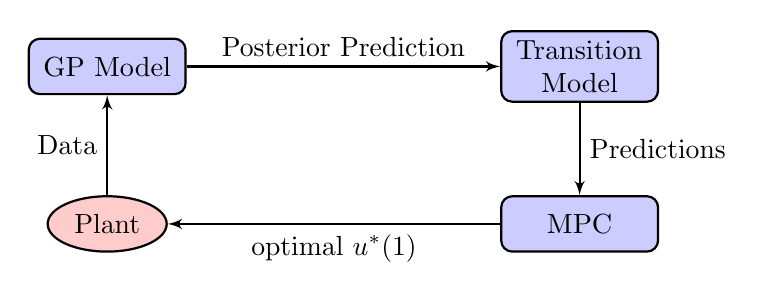
\begin{tikzpicture}[node distance=2cm, auto, thick, >=triangle 45]

    % Define block styles
    \tikzstyle{block} = [rectangle, draw, fill=blue!20, 
        text width=5em, text centered, rounded corners, minimum height=2em]
    \tikzstyle{line} = [draw, -latex']
    \tikzstyle{cloud} = [draw, ellipse,fill=red!20, minimum height=2em]

    % Define nodes
    \node [cloud] (plant) {Plant};
    % \node [block, right of=plant, node distance=4cm] (data) {Data};
    \node [block, above of=plant, node distance=2cm] (gpmodel) {GP Model};
    \node [block, right of=gpmodel, node distance=6cm] (transition) {Transition Model};
    % \node [block, below of=posterior, node distance=3cm] (transition) {Transition Model};
    \node [block, below of=transition, node distance=2cm] (mpc) {MPC};

    % Draw edges
    \path [line] (plant) -- node {Data} (gpmodel);
    % \path [line] (data) -- (gpmodel);
    \path [line] (gpmodel) -- node {Posterior Prediction} (transition);
    % \path [line] (posterior) -- (transition);
    \path [line] (transition) -- node {Predictions}(mpc);
    \path [line] (mpc) -- node {optimal $u^*(1)$}  (plant);
    
\end{tikzpicture}
\end{frame}

% \begin{frame}     \frametitle{Approach}


% % % 
% %  \begin{figure}[ht]		% h - here, t - top, b - bottom, p - page, ! - try hard
% %   \centering
% %   \afig{0.7}{figures/introduction/blockdia}			% {scaling}{Figure from MATLAB, picture, etc.}
% %   \caption{Block Diagram of GP-MPC Controller Framework}
% %   \label{f:figure1}
% % \end{figure}

% \end{frame}



%%#########################  Content ###########################################
\part{Content}

% \section{Agenda}
% \label{sec:agenda}

\begin{frame}<beamer>{Contents}
    \tableofcontents[part=2,hideallsubsections]
\end{frame}

\section{Gaussian Process }
\begin{frame}    \frametitle{Gaussian Process \cite{quinnonero2007approximation}}
    \textbf{Definition :} A Gaussian process (GP) is a collection of random variables, any finite number of which have consistent joint Gaussian distributions. \\
    % It is a Bayesian approach that assumes a GP prior over functions \cite{quinnonero2007approximation}. \\ 
    \begin{itemize}
        \item The parameter space is denoted by \( \mathcal{X} \), for example, \( \mathcal{X} \subset \mathbb{R}^D \).
        \item Evaluation points \( x^* \in \mathcal{X} \) and  \( f^* = f(x^*) \).
        \item Gaussian multivariate distribution: \(f^* \sim \mathcal{N}(\mu, \Sigma)\)
        % \item squared exponential (SE) kernel\[k(x, x') = \sigma^2 \exp \left( -\frac{(x - x')^2}{2\ell^2} \right)\] 
    \end{itemize}
     

    
    % i.e., assumes a prior that function values behave according to
    % \begin{equation}\label{eq:prior_function}
    %     p(f | x_1, x_2, \ldots, x_n) = \mathcal{N} (0, K(\mathbf{x_1},  \mathbf{x_2})), 
    % \end{equation}
    % where $f = [f_1, f_2, \ldots, f_n]^{\top}$ is a vector of latent function values, $f_i = f(\mathbf{x_i})$, and $K(\mathbf{x_1}, \mathbf{x_2})$ is a covariance matrix, whose entries are given by the covariance function, $K(\mathbf{x_1}, \mathbf{x_2})_{ij} = k(\mathbf{x_i}, \mathbf{x_j})$.
    % \begin{equation}\label{eq:covariance_function}
    %     K_{ij} = k(\mathbf{x_i}, \mathbf{x_j}) = \sigma_f^2 \exp\left( -\frac{(\mathbf{x_i} - \mathbf{x_j})^2}{2l^2} \right),
    % \end{equation}
    % where $\sigma_f^2$ controls the prior variance, and $l$ is an isotropic lengthscale parameter that controls the rate of decay of the covariance
   
    \begin{figure}[!tbp]
        \centering
        \subfloat{\includesvg[width=0.31\columnwidth]{figures/GP/ML_pre}\label{fig:f1}}
        \centering
        \subfloat{\includesvg[width=0.33\columnwidth]{figures/GP/GP_pr}\label{fig:f1}}
        \hfill
        \subfloat{\includesvg[width=0.33\columnwidth]{figures/GP/GD_pr}\label{fig:f2}}
    \end{figure}
    
\end{frame}	


%@222222222
\begin{frame}{Gaussian Process Regression}
\begin{itemize}
\item Consider the parameter space \( \mathcal{X} = [0, 5] \) and sample points 
\(x^* = [0;1]^T \) , \( f(x^*) = [0;0] \), So \( \mu = [0;0]^T \)
\item squared exponential (SE) kernel \[k(x, x') = \sigma^2 \exp \left( -\frac{(x - x')^2}{2\ell^2} \right)\] 
\item assume \(\sigma^2 = 1, \ell =1\), SE covariance function \[
\Sigma = 
\begin{pmatrix}
k(x_1, x_1) & k(x_1, x_2) \\
k(x_2, x_1) & k(x_2, x_2)
\end{pmatrix} =
\begin{pmatrix}
1 & 0.607 \\
0.607 & 1
\end{pmatrix}
\]
\item Gaussian Prior \(\mathcal{N}\left(\begin{bmatrix}0 \\0\end{bmatrix}, \begin{bmatrix}1 & 0.607 \\0.607 & 1 \end{bmatrix}\right)\)
\end{itemize}
\end{frame}

%33333333333
% \begin{frame}{Gaussian Process Regression}
%     \begin{itemize}
%         \item Ex 1, \(x^* = [0,1]^T \) , \( f(x^*) = [0, 0] \), \(\mathcal{N}\left(\begin{bmatrix}0 \\0\end{bmatrix}, \begin{bmatrix}1 & 0.607 \\0.607 & 1 \end{bmatrix}\right)\)
%         \item Ex 2, \(x^* = [0,2]^T \) , \( f(x^*) = [0, 1] \), \(\mathcal{N}\left(\begin{bmatrix}0 \\1\end{bmatrix}, \begin{bmatrix}1 & 0.135 \\0.135 & 1 \end{bmatrix}\right)\)
%     \end{itemize}
%         \begin{figure}[!tbp]
%         \centering
%         \includesvg[width=0.6\columnwidth]{figures/GP/bivariateGD}\label{fig:f1}
%     \end{figure}
    
% \end{frame}



% \begin{frame}{Frame Title}

%     \begin{figure}[!tbp]
%         \centering
%         \subfloat{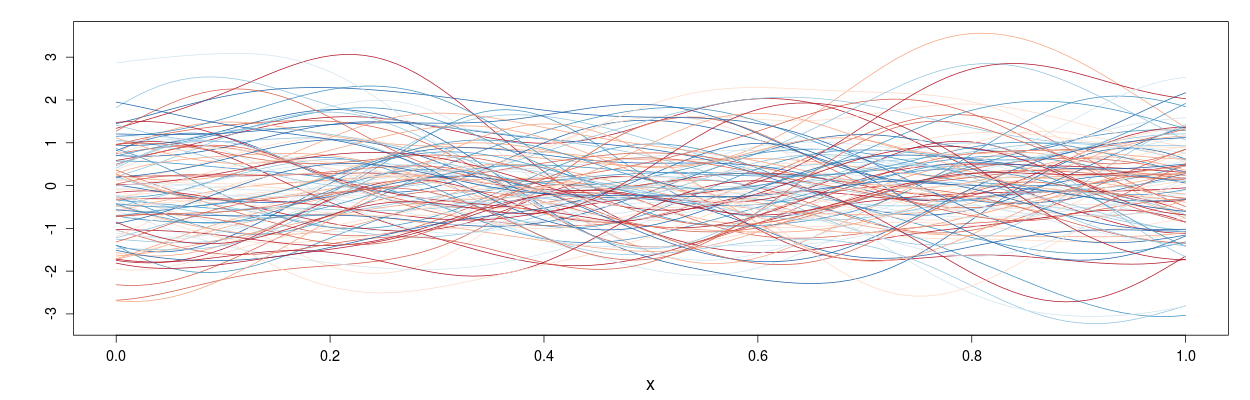
\includegraphics[width=1\textwidth]{figures/GP/download.png}\label{fig:f1}}
%         \hfill
%         \subfloat{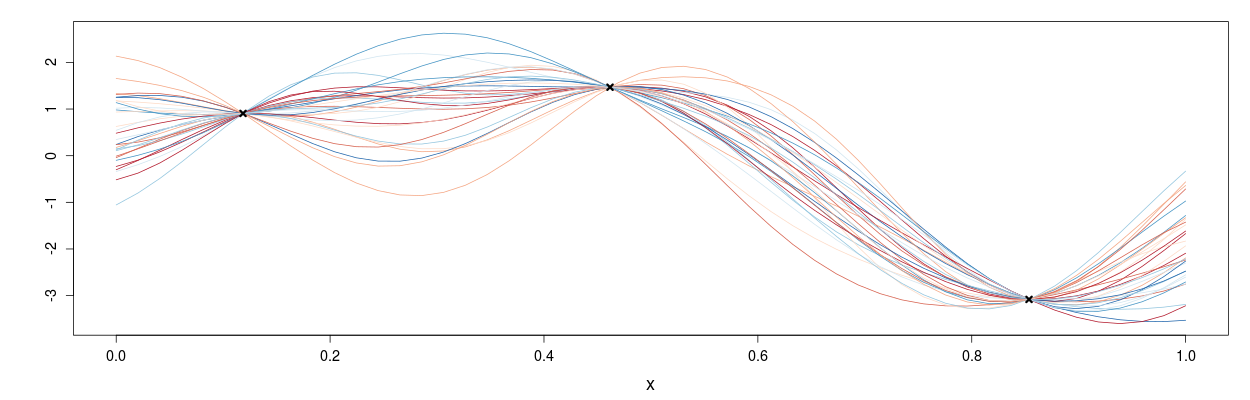
\includegraphics[width=1\textwidth]{figures/GP/posterior1.png}\label{fig:f2}}
%     \end{figure}
% \end{frame}

\begin{frame}{Observation}
    \begin{itemize}
    \item Training points \( x \) and observations \( f(x) \).
    
    \item Noisy observations are given by:\(y = f(x) + \omega\) where \( \omega \) is independent Gaussian noise with variance \( \sigma_n^2 \).
    
    \item The covariance of \( y \) is: \(\text{cov}(y) = k(X, X') + \sigma_n^2 I\)
    
    \item The joint distribution  \(\begin{bmatrix}y \\f^*\end{bmatrix}\sim \mathcal{N} \left(\begin{bmatrix}\mu \\ \mu^* \end{bmatrix},\begin{bmatrix}
    K(X, X) + \sigma_n^2 I & K(X, X^*) \\ K(X^*, X) & K(X^*, X^*) \end{bmatrix} \right)
    \)
    
    \item \( f^* | X^*, X, y\sim \mathcal{N} (\mu^* + K(X, X^*) ( K(X, X) + \sigma_n^2 I)^{-1} (y - \mu), \\ \qquad \quad \qquad \quad K(X^*, X^*) - K(X^*, X) ( K(X, X) + \sigma_n^2 I )^{-1} K(X, X^*) )
    \)

\end{itemize}
\end{frame}

\begin{frame}{Graphical Interpretation}

    \begin{figure}[!tbp]
        \centering
        \includesvg[width=0.6\columnwidth]{figures/GP/GP_PP}\label{fig:f1}
    \end{figure}
\end{frame}


\begin{frame}{Hyper parameters}
        \begin{figure}[!tbp]
        \centering
        \subfloat{\includesvg[width=0.25\columnwidth]{figures/GP/hyp_1}\label{fig:f1}}
        \centering
        \subfloat{\includesvg[width=0.25\columnwidth]{figures/GP/hyp_2}\label{fig:f1}}
        \centering
        \subfloat{\includesvg[width=0.25\columnwidth]{figures/GP/hyp_3}\label{fig:f2}}
        \hfill
        \subfloat{\includesvg[width=0.25\columnwidth]{figures/GP/hyp_11}\label{fig:f1}}
        \centering
        \subfloat{\includesvg[width=0.25\columnwidth]{figures/GP/hyp_3}\label{fig:f1}}
        \centering
        \subfloat{\includesvg[width=0.25\columnwidth]{figures/GP/hyp_13}\label{fig:f2}}
    \end{figure}
\end{frame}





% \begin{frame}	\frametitle{Linear Regression GP Model}
%     Probabilistic regression is usually formulated as follows: given a training set $D = \{(\mathbf{x_i}, y_i), i = 1, \ldots, n\}$ of $n$ pairs of (vectorial) inputs $\mathbf{x_i}$ and noisy (real, scalar) outputs $y_i$, compute the predictive distribution of the function values $f^*$ (or noisy $y^*$) at test locations $\mathbf{x^*}$.
    
%     we assume that the noise is additive, independent, and Gaussian, such that the relationship between the (latent) function f(x) and the observed noisy targets y is given by,
%     \begin{equation}\label{eq:latent_function}
%     \begin{aligned}
%         f(x_i) &= \mathbf{x_i}^T \mathbf{w}, \, \, \,\, \, \,\,\, \,\,\,\,\,\,\,\,\, \, y_i &= f(\mathbf{x_i}) + \epsilon_i
%     \end{aligned}
%     \end{equation}
%     where $\mathbf{w} \in \mathbb{R}^D$ is the weight column vector of the linear model, $\mathbf{x}$ is the input vector,  $\epsilon_i \sim \mathcal{N}(0, \sigma^2_{\text{noise}})$, and $\sigma^2_{\text{noise}}$ is the variance of the noise and $y$ is the observed value.
%     The noise $\epsilon$ is assumed to be zero-mean with variance $\sigma^2_n$, thus $\epsilon \sim \mathcal{N}(0, \sigma^2_n)$ 
% \end{frame}	

% \begin{frame}       \frametitle{Posterior Distribution}
%     \begin{itemize}
%         \item The posterior distribution is the updated distribution after incorporating the training data.
%         \item It combines the prior distribution and the likelihood of the observed data.
%         \item The posterior is distributed according to:
    
%     \begin{equation}\label{eq:posterior_distrubtion}
%         p(\mathbf{w | y}, X) = \mathcal{N}\left(\frac{1}{\sigma^2_n} A^{-1} X\mathbf{y}, A^{-1}\right)
%     \end{equation}
%     Where $A = \sigma^{-2}_n XX^T + \Sigma^{-1}_p$
%     \end{itemize}
% \end{frame}

% \begin{frame}

%     \begin{figure}[!tbp]
%         \centering
%         \subfloat[Prior]{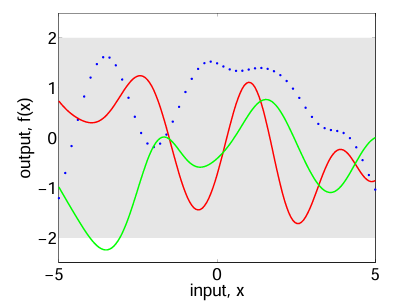
\includegraphics[width=0.5\textwidth]{figures/GP/prior.png}\label{fig:f1}}
%         \hfill
%         \subfloat[Posterior]{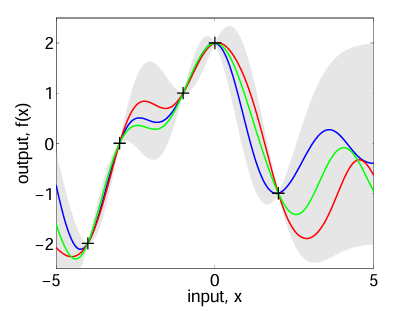
\includegraphics[width=0.5\textwidth]{figures/GP/posterior.png}\label{fig:f2}}
%         \caption{Panel (a) displays three functions drawn at random from a GP prior.  Panel (b) illustrates three random functions drawn from the posterior \cite{williams2006gaussian}.}
%     \end{figure}
% \end{frame}

% \begin{frame}{Prediction with noise-free observations}
%     For noise-free observations $\{(\mathbf{x_i}, f_i) | i = 1,...,n\}$ and test points \( X^* \), the joint distribution of training outputs $f$ and test outputs $f^*$ under the prior is given by:
%     \begin{equation}\label{eq:noisefree_joint_distrubtion}
%         \begin{bmatrix}f, f^*\end{bmatrix} \sim \mathcal{N} \left(0, \begin{bmatrix} K(X,X) & K(X,X^*) \\ K(X^*,X) & K(X^*,X^*) \end{bmatrix} \right)
%     \end{equation}
%     The resulting posterior distribution is expressed as:
%         \begin{align}\label{noisefree_predictive_distrbution}
%         \bar{f}^* &=K(X^*,X)K(X,X)^{-1}f \\
%         \text{cov}(f^*) &= K(X^*,X^*) - K(X^*,X)K(X,X)^{-1}K(X,X^*)
%     \end{align}

% \end{frame}

% \begin{frame}{Prediction with noisy observations}
%     Prediction with noisy observations incorporates additive independent identically distributed Gaussian noise. The joint distribution of observed target values and function values at test locations under the prior is given by:

%     \begin{equation}\label{eq:noisy_joint_distrubtion}
%         \begin{bmatrix}\mathbf{y}, f^* \end{bmatrix} \sim \mathcal{N} \left(0, \begin{bmatrix} K(X,X) + \sigma^2_n I & K(X,X^*) \\ K(X^*,X) & K(X^*,X^*) \end{bmatrix} \right)
%     \end{equation}

%     The predictive equations for GP regression are:
%     \begin{align}\label{noisy_predictive_distrbution}
%         \bar{f}^* &= K(X^*,X)[K(X,X) + \sigma^2_n I]^{-1}y \\
%         \text{cov}(f^*) &= K(X^*,X^*) - K(X^*,X)[K(X,X) + \sigma^2_n I]^{-1}K(X,X^*)
%     \end{align}
%     These equations provide mean predictions and uncertainties for test targets.
% \end{frame}

% \begin{frame}{Extension to Non-Linear Functions}
%     \begin{itemize}
%         \item Non-linearity between input and output variables
%         \item Poor predictions and biased estimates if linear model is used
%         \item The order of the target function is generally unknown, direct application of raw inputs is not effective.
%     \end{itemize}
%     To overcome above problem, the idea is to transform the inputs into a higher dimensional space via basis functions $\psi(x)$, $\psi : \mathbb{R}^D \rightarrow \mathbb{R}^N$, where $N \gg D$, and then apply the linear regression model. Thus the linear regression model Equation \ref{eq:latent_function} is reformulated such that 
%     \begin{equation}\label{eq:non_linear_regression_model}
%         f(x) = \psi(x)w, \quad 
%     \end{equation}
% \end{frame}

% \begin{frame}
%     Accordingly, the predictive distribution is given by:

% \begin{equation}\label{eq:Nl_pd}
% p(f^*|X^*,X,\mathbf{y}) = \mathcal{N} \left( \frac{1}{\sigma_n^2} \Psi(X^*)^T A^{-1} \Psi(X) \mathbf{y}, \frac{1}{\sigma_n^2} \Psi(X^*)^T A^{-1} \Psi(X^*) \right)
% \end{equation}
% With $A = \sigma^{-2} n \Psi(X)\Psi(X)^T + \Sigma_p$, can be rearranged as shown in \cite{williams2006gaussian}, such that

% \begin{equation}\label{eq:NL_pd_arranged}
%  = \mathcal{N}(\Psi_*^T \Sigma_p \Psi_K + \sigma^2_n I)^{-1} y, \Psi_*^T \Sigma_p \Psi_* - \Psi_*^T \Sigma_p \Psi_K + \sigma^2_n I)^{-1} \Psi_*^T \Sigma_p \Psi_*,
% \end{equation}

% where $K = \Psi_*^T \Sigma_p \Psi$.
% Defining $\varphi(x) = \Sigma_{1/2}^p \psi(x)$ (notice that $\Sigma_p$ is positive definite), the expressions can be substituted by $\varphi(x) \varphi(x)^T$. So $\langle \varphi(x), \varphi(x)^T \rangle$ can be replaced by kernel function $k(x,x^T)$ using Mercer’s theorem \cite{kanagawa2018}. 

% \end{frame}

% \begin{frame}
%     The kernel matrices $K(\cdot,\cdot)$ which are given by:
% \begin{equation}\label{eq:kernal_f}
%     K(X,Y) =
% \begin{pmatrix}
% k(X_1,Y_1) & \cdots & k(X_1,Y_M) \\
% \vdots & \ddots & \vdots \\
% k(X_N,Y_1) & \cdots & k(X_N,Y_M)
% \end{pmatrix}
% \end{equation}

% Substituting kernal function (\ref{eq:kernal_f}) into (\ref{eq:NL_pd_arranged})

% \begin{equation}\label{eq: NL_pd_implicit}
% \begin{aligned}
% p(f^*|X^*,X,\mathbf{y}) & = \mathcal{N} (K(X^*,X) [K(X,X) + \sigma^2_n I]^{-1} y,  \nonumber \\
% & \qquad  K(X^*,X^*) - K(X^*,X)[K(X,X) + \sigma^2_n I]^{-1} K(X,X^*)).
% \end{aligned}
% \end{equation}
% \end{frame}





%%%%%%%%%%%%%%%%%%%%%%%%%%%%%%%%%%%%%%%%%%%%%%%%%%%%%%%%%%%%%%%%%%%%%%%%%%%%%%%%%%%%%%%%%%%%%





\begin{frame}{Optimization of the Hyperparameters\cite{Lubsen2022}}
    \begin{itemize}
        \item Necessary to the use of computationally efficient optimization methods.
        \item Two such methods are maximizing the marginal likelihood and cross-validation. %\cite{williams2006gaussian}.
        \item In marginal liklihood, the gradient-based algorithm is used.
%          Depending on the initial value, a gradient-based
% optimizer will converge to one of the optima. Therefore, the hyperparameters should
% be chosen reasonably. Another possibility is the utilization of 
% \item Global optimizers such as Dividing Rectangles (DIRECT) is a gradient free optimization algorithm that performs very well for low-dimensional problems
\begin{figure}
    \centering
    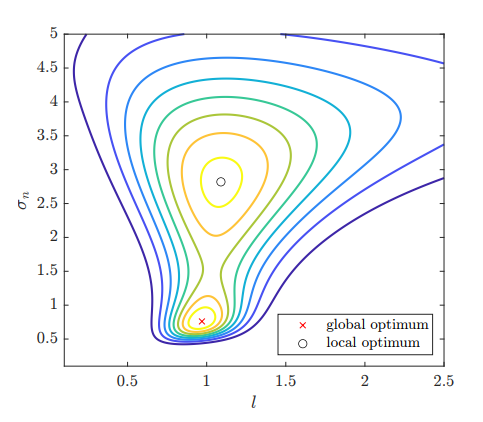
\includegraphics[width=0.35\linewidth]{figures/GP/Contour_hyp.png}
    % \caption{Contour of the marginal likelihood depending on the length scale \( l \) and noise \( \sigma_n \) \cite{Lubsen2022}.}
    \label{fig:opt_hyp_post}

    %Note : question noise
\end{figure}


% \begin{equation}
% p(w \mid y, X, \theta) = \frac{p(y \mid X, w, \theta) \cdot p(w \mid \theta)}{p(y \mid X, \theta)}
% \end{equation}

% By conditioning with \(\theta\). The denominator is the marginal likelihood and is independent of the parameters. It can be determined by integration of the product of the likelihood and the prior over the model parameters:

% \begin{equation} \label{eq: marginal_likelihood}
% p(y \mid X, \theta) = \int p(y \mid X, w, \theta) \cdot p(w \mid \theta) \, dw.
% \end{equation}

    \end{itemize}
\end{frame}


%%%%%%%%%%%%%%%%%%%%%%%%%%%%%%%%%%%%%%%%%%%%%%%%%%%%%%%%%%%%%%%%%%%%%%%%%%%%%%%%%


\begin{frame}{Long-term Prediction}
    % When the input \( X^* \) is a deterministic input, the mean and covariance of the prediction are calculated according Joint distribution eq. However, if the input itself is Gaussian, \( X \sim \mathcal{N}( \bar{x^*}, \Sigma_x^* ) \), the predictive distribution becomes:

    \begin{equation}\label{eq:single_prediciton}
        p(f^*|\mu_x^*, \Sigma_x^* , \mathbf{D}) = \int p(f^*|X^*, \mathbf{D}) \cdot p(X^*|\Sigma_x^* , \mathbf{D}) \, dx^* \quad
    \end{equation}

    \begin{itemize}
        \item The integral is analytically intractable. %\cite{hewing2017cautious}.
        \item Approximate the integral numerically using Monte-Carlo methods. %\cite{girard2002gaussian}.
        \item To approximate the posterior distribution as a Gaussian by calculating its mean and variance (Moment Matching).

    \end{itemize}

\end{frame}

\begin{frame}{Moment Matching Approximation \cite{deisenroth2011pilco}}
    \begin{figure}
    \centering
    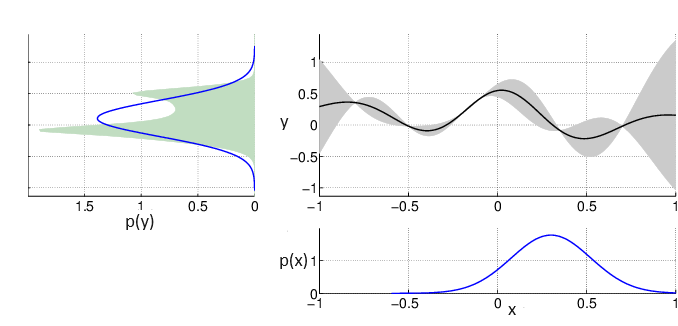
\includegraphics[width=1\linewidth]{figures/GP/MM_GP.png}
    % \caption{Contour of the marginal likelihood depending on the length scale \( l \) and noise \( \sigma_n \) \cite{Lubsen2022}.}
    \label{fig:mm}

    %Note : question noise
\end{figure}
\end{frame}

% \begin{frame}{Moment Matching Approximation}

% \begin{itemize}
%     \item Alternatively, the posterior distribution \( p(f|x, \mathbf{X}, \mathbf{D}) \) can be approximated as a Gaussian by calculating its mean and variance.
%     \item Several methods exist for this Gaussian approximation, such as Moment Matching and linearization of the posterior GP mean function\cite{marc2015robotics}.
%     \item Moment Matching computes the first two moments of the predictive distribution exactly, whereas linearization provides a computationally efficient approximation by explicitly linearizing the posterior GP.
%     \item Moment Matching is better than linearization, we will focus on the Moment Matching Gaussian approximation.
% \end{itemize}
% \end{frame}

% \begin{frame}{Mean Prediction}
%     Following the law of iterated expectations, for target dimensions \( a = 1,..., D \) we obtain the predictive mean:

% \begin{equation}\label{eq:mu}
% \begin{aligned}
% \mu_t^a & =\mathbb{E}_{\tilde{\boldsymbol{x}}_{t-1}}\left[\mathbb{E}_{f_a}\left[f_a\left(\tilde{\boldsymbol{x}}_{t-1}\right) \mid \tilde{\boldsymbol{x}}_{t-1}\right]\right]=\mathbb{E}_{\tilde{\boldsymbol{x}}_{t-1}}\left[m_{f_a}\left(\tilde{\boldsymbol{x}}_{t-1}\right)\right] \\
% & =\int m_{f_a}\left(\tilde{\boldsymbol{x}}_{t-1}\right) \mathcal{N}\left(\tilde{\boldsymbol{x}}_{t-1} \mid \tilde{\boldsymbol{\mu}}_{t-1}, \tilde{\boldsymbol{\Sigma}}_{t-1}\right) d \tilde{\boldsymbol{x}}_{t-1} \\
% & =\boldsymbol{\beta}_a^T \boldsymbol{q}_a 
% % \boldsymbol{\beta}_a & =\left(\boldsymbol{K}_a+\sigma_{w_a}^2\right)^{-1} \boldsymbol{y}_a
% \end{aligned}
% \end{equation}
% where, \quad $\boldsymbol{\beta}_a =\left(\boldsymbol{K}_a+\sigma_{w_a}^2\right)^{-1} \boldsymbol{y}_a ,$ \quad \quad $
%   \boldsymbol{q}_a=\left[q_{a_1}, \ldots, q_{a_n}\right]^T$. 
% \begin{equation}\label{eq:mu_qa}
% \begin{aligned}
% q_{a_i} & =\int k_a\left(\tilde{\boldsymbol{x}}_i, \tilde{\boldsymbol{x}}_{t-1}\right) \mathcal{N}\left(\tilde{\boldsymbol{x}}_{t-1} \mid \tilde{\boldsymbol{\mu}}_{t-1}, \tilde{\boldsymbol{\Sigma}}_{t-1}\right) d \tilde{\boldsymbol{x}}_{t-1} \\
% & =\sigma_{f_a}^2\left|\tilde{\boldsymbol{\Sigma}}_{t-1} \boldsymbol{\Lambda}_a^{-1}+\boldsymbol{I}\right|^{-\frac{1}{2}} \exp \left(-\frac{1}{2} \boldsymbol{\nu}_i^T\left(\tilde{\boldsymbol{\Sigma}}_{t-1}+\boldsymbol{\Lambda}_a\right)^{-1} \boldsymbol{\nu}_i\right),
% \end{aligned}
% \end{equation}

% where we define
% \begin{equation}\label{eq:difference_vi}
%     \nu_i:=\left(\tilde{\boldsymbol{x}}_i-\tilde{\boldsymbol{\mu}}_{t-1}\right)
% \end{equation}
% \end{frame}


% \begin{frame}{Covariance Matrix Prediction}
%     The Predictive covariance matrix $\mathbf{\Sigma}_{\Delta} \in \mathbb{R}^{D \times D}$ is given by 
%     \begin{equation}
%     \sum (:) = 	\begin{bmatrix}
%                         \sigma_{a a}^2 & \sigma_{a b}^2 &......\\
%                         \sigma_{a b}^2 & \sigma_{b b}^2 &......\\
%                         .&.& ......\\
%                         .&.& ......\\
%                         \end{bmatrix}_{DxD}
% \end{equation}
% where, 
% \begin{equation}\label{eq:sigma_aa}
% \sigma_{a a}^2  =\mathbb{E}_{\overline{\boldsymbol{x}}_t}\left[\operatorname{var}_f\left[\Delta_a \mid \tilde{\boldsymbol{x}}_t\right]\right]+\mathbb{E}_{f, \overline{\boldsymbol{x}}_t}\left[\Delta_a^2\right]-\left(\boldsymbol{\mu}_{\Delta}^a\right)^2,
% \end{equation}
% \begin{equation}\label{eq:sigma_ab}
%     \sigma_{a b}^2 =\mathbb{E}_{f, \overline{\boldsymbol{x}}_t}\left[\Delta_a \Delta_b\right]-\boldsymbol{\mu}_{\Delta}^a \boldsymbol{\mu}_{\Delta}^b, \quad a \neq b,
% \end{equation}

% \begin{equation}\label{eq:Eab}
% \begin{aligned}
% \mathbb{E}_{f, \overline{\boldsymbol{x}}_t}\left[\Delta_a \Delta_b\right] & =\mathbb{E}_{\overline{\boldsymbol{x}}_t}\left[\mathbb{E}_f\left[\Delta_a \mid \tilde{\boldsymbol{x}}_t\right] \mathbb{E}_f\left[\Delta_b \mid \tilde{\boldsymbol{x}}_t\right]\right] \\
% & {=} \int m_f^a\left(\tilde{\boldsymbol{x}}_t\right) m_f^b\left(\tilde{\boldsymbol{x}}_t\right) p\left(\tilde{\boldsymbol{x}}_t\right) \mathrm{d} \tilde{\boldsymbol{x}}_t \\
% & =\boldsymbol{\beta}_a^{\top} \boldsymbol{Q} \boldsymbol{\beta}_b,
% \end{aligned}
% \end{equation}
% \end{frame}

% \begin{frame}{Covariance Matrix Prediction}
    
% \begin{equation}\label{eq:Q_integral}
%     \boldsymbol{Q}:=\int k_a\left(\tilde{\boldsymbol{x}}_t, \tilde{\boldsymbol{X}}\right)^{\top} k_b\left(\tilde{\boldsymbol{x}}_t, \tilde{\boldsymbol{X}}\right) p\left(\tilde{\boldsymbol{x}}_t\right) \mathrm{d} \tilde{\boldsymbol{x}}_t .
% \end{equation}

% Using standard results from Gaussian multiplications and integration, we obtain the entries $Q_{i j}$ of $Q \in \mathbb{R}^{n \times n}$
% \begin{equation}\label{eq:Qij}
%     Q_{i j}=|\boldsymbol{R}|^{-\frac{1}{2}} k_a\left(\tilde{\boldsymbol{x}}_i, \tilde{\boldsymbol{\mu}}_t\right) k_b\left(\tilde{\boldsymbol{x}}_j, \tilde{\boldsymbol{\mu}}_t\right) \exp \left(\frac{1}{2} \boldsymbol{z}_{i j}^{\top} \boldsymbol{T}^{-1} \boldsymbol{z}_{i j}\right)
% \end{equation}

% where we define
% $\qquad \boldsymbol{R}  :=\tilde{\boldsymbol{\Sigma}}_t\left(\boldsymbol{\Lambda}_a^{-1}+\boldsymbol{\Lambda}_b^{-1}\right)+\boldsymbol{I}, \qquad \boldsymbol{T}:=\boldsymbol{\Lambda}_a^{-1}+\boldsymbol{\Lambda}_b^{-1}+\tilde{\boldsymbol{\Sigma}}_t^{-1}, \\ \boldsymbol{z}_{i j} :=\boldsymbol{\Lambda}_a^{-1} \boldsymbol{\nu}_i+\boldsymbol{\Lambda}_b^{-1} \boldsymbol{\nu}_j,$

% From (\ref{eq:sigma_aa}), we see that the diagonal entries contain the additional term
% \begin{equation}\label{eq:E_xa}
% \mathbf{E}_{\overline{\boldsymbol{x}}_t}\left[\operatorname{var}_f\left[\Delta_a \mid \tilde{\boldsymbol{x}}_t\right]\right]=\sigma_{f_a}^2-\operatorname{tr}\left(\left(\boldsymbol{K}_a+\sigma_{w_a}^2 \boldsymbol{I}\right)^{-1} \boldsymbol{Q}\right)+\sigma_{w_a}^2
% \end{equation}
%  $\sigma_{w_a}^2$ being the system noise variance of the $a$th target dimension. 
% \end{frame}

%%%%%%%%%%%%%%%%%%%%%%%%%%%%%%%%%%%%%%%%%%%%%%%%%%%%%%%%%%%%%%%%%%%%%%%%%%%%%%%%%%%%%%%%%%%%%%%%%%%%


% \begin{frame}
%     The optimal solution would be a predictive distribution without dependency on the hyperparameters. By marginalization of \( \theta \), a hyperparameter-independent formalism can be obtained:

% \begin{equation}\label{eq: predictive_distribution}
% p(f^*|y,X,X^*) = \int p(f^*|y,\theta,X,X^*) \cdot p(y|\theta,X,X^*) \cdot p(\theta|X,X^*) \, d\theta.
% \end{equation}

% Unfortunately, this integral is not analytically tractable, and has non-trivial dependencies on \( \theta \). Several methods exist to estimate the integral, such as Hamiltonian Monte Carlo (HMC), Bayesian Monte Carlo (BMC), and Sequential Monte Carlo (SMC).

% An alternative approach to approximate \eqref{eq: predictive_distribution} is by maximizing the second-level marginal likelihood (ML-II) given by \eqref{eq: marginal_likelihood}. As shown in previous work, finding the hyperparameters \( \theta_{\text{max}} \) that maximize \( p(y|X,\theta) \) leads to:
% \[
% p(f^*|y,X,X^*) \approx p(f^*|\theta_{\text{max}},y,X,X^*).
% \]
% \end{frame}

% \begin{frame}
%     \begin{itemize}
%         \item This method offers the advantage of analytically tractable integration.
%         \item Gradient-based algorithms are typically used for maximization. It is highly sensitive to initial values.
%         \item The non-convex nature of the marginal likelihood surface can lead to overfitting or underfitting.
%         \item Global optimization using the hyperparameters at the global optimum results in preferable predictions compared to local minima, where observations may be misinterpreted as noise.
%         \item Alternative methods such as global optimizers like Dividing Rectangles (DIRECT) can be utilized to mitigate sensitivity to initial values.
%     \end{itemize}
% \end{frame}

% \begin{frame}
%     \begin{figure}
%     \centering
%     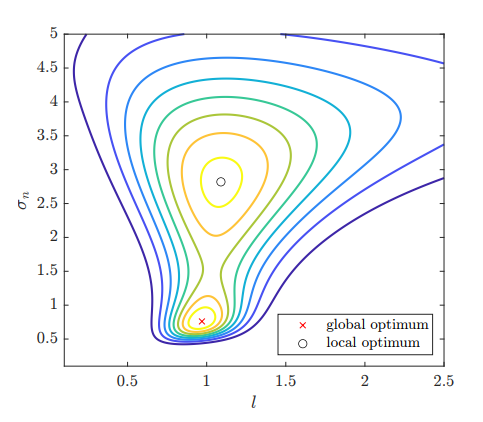
\includegraphics[width=0.75\linewidth]{figures/GP/Contour_hyp.png}
%     \caption{Contour of the marginal likelihood depending on the length scale \( l \) and noise \( \sigma_n \) \cite{Lubsen2022}.}
%     \label{fig:opt_hyp_post}

%     %Note : question noise
% \end{figure}
% \end{frame}



% \begin{frame}	\frametitle{Nonpredictive Scenario (by AT) - Simulink}
% 		\centering
% 		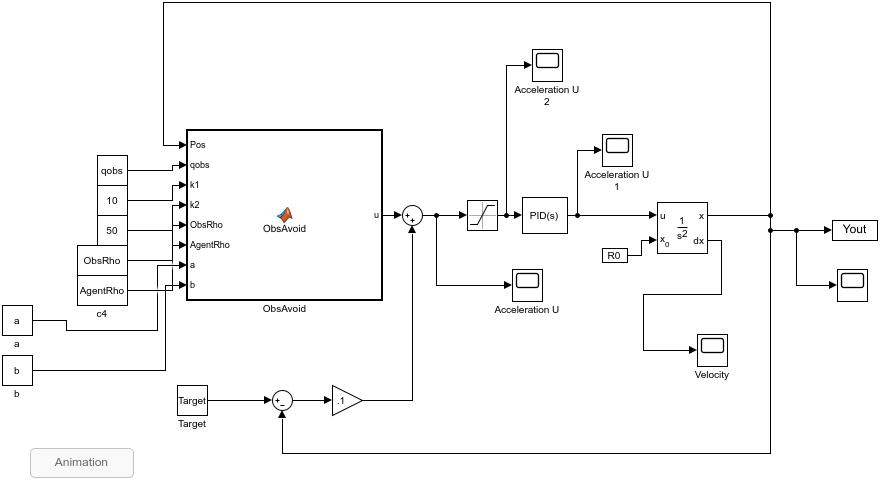
\includegraphics[scale=0.7, angle=0]{tmp30938.jpg}
% \end{frame}

\section{MPC and GP-MPC Learning}

\begin{frame}{Model Predicitve control}
    \begin{itemize}
        \item Model Predictive Control (MPC) is an advanced control method that uses a model of the system to predict and optimize the control actions over a future time horizon.
        % \item MPC relies on a dynamic model of the process being controlled.
        \item MPC operates on a receding horizon principle 
        % where it repeatedly solves a finite horizon optimal control problem (OCP) at each time step.
        \item directly address State and input constraints
        % Unlike many other control methods, MPC can directly address constraints on the input, state, and output during the design process, enhancing its applicability in practical scenarios.
        \item the high computational cost of solving the OCP
        % One of the main challenges of MPC is the high computational cost of solving the OCP within the sampling time.

        
    \end{itemize}
     \begin{figure}[ht]		% h - here, t - top, b - bottom, p - page, ! - try hard
        \centering
        \afig{0.5}{figures/GP/mpc}			% {scaling}{Figure from MATLAB, picture, etc.}
        \caption{MPC Illustration\cite{maiworm2021gaussian}}
        % \caption{MPC Illustration: For a particular initial condition $x_k$ at time instant $k$, a predicted open-loop sequence of inputs $\hat{u}$ is computed up to a prediction horizon $N$. The input sequence, together with the resulting predicted states $\hat{x}$, are computed in such a way that they minimize a given cost\cite{maiworm2021gaussian}.}
        \label{f:figure_mpc}
    \end{figure}
\end{frame}




% \begin{frame}{Model Predicitve control \cite{maiworm2021gaussian}}
%      \begin{figure}[ht]		% h - here, t - top, b - bottom, p - page, ! - try hard
%         \centering
%         \afig{0.9}{figures/GP/mpc}			% {scaling}{Figure from MATLAB, picture, etc.}
%         % \caption{MPC Illustration: For a particular initial condition $x_k$ at time instant $k$, a predicted open-loop sequence of inputs $\hat{u}$ is computed up to a prediction horizon $N$. The input sequence, together with the resulting predicted states $\hat{x}$, are computed in such a way that they minimize a given cost\cite{maiworm2021gaussian}.}
%         \label{f:figure_mpc}
%     \end{figure}
% \end{frame}





% \begin{frame}{Model Predicitve control}
%     The basic procedure applied by a model predictive control scheme can be illustrated in Figure \ref{f:figure_mpc} and summarized as follows:

%     \begin{enumerate}
%         \item Obtain the state $x_k$ at the current time step $k$.
%         \item Formulate and solve a finite horizon optimal control problem. This involves predicting the future evolution of the system and determining an optimal input sequence that minimizes a given cost function over a finite prediction horizon.
%         \item Apply the first part of the optimal input sequence to the system. 
%         \item Repeat, go back to Step 1.
%     \end{enumerate}
% \end{frame}





\begin{frame}{GP-MPC framework}
    \centering
    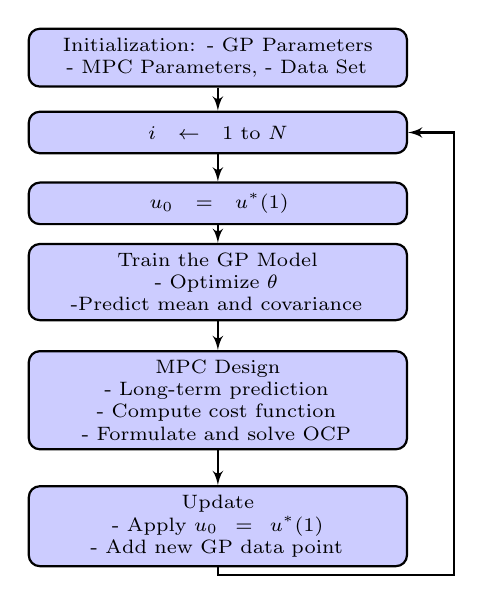
\begin{tikzpicture}[node distance=2cm, auto, thick, >=triangle 45]
    % Define block styles
    \tikzstyle{block} = [rectangle, draw, fill=blue!20, 
        text width=13em, text centered, rounded corners, minimum height=1.5em, font=\scriptsize]
    \tikzstyle{line} = [draw, -latex']
    
    % Define nodes
    \node [block] (init) {Initialization: - GP Parameters\\- MPC Parameters,  - Data Set};
    \node [block, below of=init, node distance=0.95cm] (recursion) { $i \leftarrow 1$ to $N$};
    \node [block, below of=recursion, node distance=0.9cm] (in) {$u_0 = u^*(1)$};
    \node [block, below of=in, node distance=1cm] (train) {Train the GP Model\\- Optimize $\theta$ \\-Predict mean and covariance};
    \node [block, below of=train, node distance=1.5cm] (mpc) {MPC Design\\- Long-term prediction\\- Compute cost function\\- Formulate and solve OCP};
    
    \node [block, below of=mpc, node distance=1.6cm] (update) {Update\\- Apply $u_0 = u^*(1)$ \\- Add new GP data point};
    
    % Draw edges
    \path [line] (init) -- (recursion);
    \path [line] (recursion) -- (in);
    \path [line] (in) -- (train);
    \path [line] (train) -- (mpc);
    \path [line] (mpc) -- (update);
    \path [line] (update.south) -- ++(0,-0.1) -| ++(3,0) |- ++(0,2) |- ++(0,2) |- (recursion.east);

    \end{tikzpicture}
\end{frame}































% \begin{frame}	\frametitle{What I want to do}
% 	\begin{itemize}
% 		\item Continue reading and filling the table
% 		\item Think about how to include consensus? (Flocking, or other ideas?!) \cite{EiHoWe13d,ElAh07}
% 		\item if using a "global" costfunction, how to cope with iterations, are they avoidable to some extent?
% 	\end{itemize}
% \end{frame}

\section{Results and Discussion}

\begin{frame}	\frametitle{Simulation Results}
	\begin{itemize}
 \item Linear system -  DC motor
 \item Non-Linear system - Van der Pol oscillator
            \item Validation of GP Model and the Moment Matching model
            \item Modeling without uncertainty
            \item Modeling with uncertainty


            
\end{itemize}
\end{frame}


\begin{frame}{DC Motor\cite{werner2023grt}}
            \begin{figure}
                \centering
                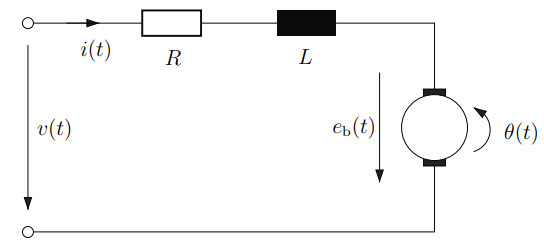
\includegraphics[width=0.6\linewidth]{figures//Results/DC_motor.png}
                \caption{DC Motor}
            \end{figure}
   \[ V(t) = L\frac{di}{dt} + R_m i(t) + K_e \omega(t) \] \\ 
     \[G(s) = \frac{21}{s(1.1s + 1)}\]

   
\end{frame}


\begin{frame}{Validation of DC Motor Learning}
     \begin{itemize}
    \item $x_1$ is the angular velocity ($\dot{\theta}$)
    \item $x_2$ is the angle ($\theta$) 
    \item control input is voltage ($v$)
    
    \end{itemize}
    \[  \dot{x} = \begin{bmatrix}
        -0.9091 & 0 \\ 
        1 & 0
    \end{bmatrix} x + \begin{bmatrix}
        4 \\ 0
    \end{bmatrix} u \] \\
   \[ y = \begin{bmatrix}
        0 & 4.7727
    \end{bmatrix} x \]

    \begin{itemize}
        \item Zoh discretization with $T_s=0.1$.
        \item initial states are $x_1 = 0$ and $x_2=\pi$
    \end{itemize}
           \[  x_{k+1} = \begin{bmatrix}
        0.9131 & 0 \\ 
        0.0956 & 1
    \end{bmatrix} x_k + \begin{bmatrix}
        0.3824 \\ 0.0194
    \end{bmatrix} u_k \] \\
     \[ yk = \begin{bmatrix}
        0 & 4.7727
    \end{bmatrix} x_k \]

%     \begin{figure}
%     \centering
%     \includesvg[width=0.6\columnwidth]{figures/DC_motor/gp_test_dc}
%     % \caption{Gaussian Process model testing of DC motor }
%     \label{fig:GP_model_testing}
    
% \end{figure}
\end{frame}

\begin{frame}{Validation of DC Motor Learning}
    \begin{figure}[!tbp]
        \centering
        \subfloat[GP model validation]{\includesvg[width=0.5\columnwidth]{figures/DC_motor/gp_test_dc}\label{fig:f1}}
        \centering
        \subfloat[Moment Matching model Validation]{\includesvg[width=0.5\columnwidth]{figures/DC_motor/long_term_test_dc}\label{fig:f1}}
    \end{figure}
%     \begin{figure}
%     \centering
%     \includesvg[width=0.8\columnwidth]{figures/DC_motor/long_term_test_dc}
%     % \caption{Longterm prediction model testing}
%     \label{fig:longterm_testing}
% \end{figure}
\end{frame}


\begin{frame}{DC Motor Without Uncertainty(Disturbances)}
    \begin{figure}[!tbp]
        \centering
        \subfloat[GP-MPC controller $t_s=8$]{\includesvg[width=0.5\columnwidth]{figures/DC_motor/gp_mpc_wo_1}\label{fig:f1}}
        \centering
        \subfloat[f-MPC controller $t_s=7$]{\includesvg[width=0.5\columnwidth]{figures/DC_motor/f_mpc_wo_dc}\label{fig:f1}}
    \end{figure}
%     \begin{figure}
%     \centering
%     \includesvg[width=0.8\columnwidth]{figures/DC_motor/gp_mpc_wo_1}
%     % \caption{GP-MPC controller- noise free DC motor plant without parameter uncertainty}
%     \label{fig:GPMPC_DC_wo_noise}
% \end{figure}
\end{frame}


\begin{frame}{DC Motor With Uncertainty(Disturbances)}
\begin{itemize}
        \item Uncertainty Model
    \end{itemize}
     \[ x_{k+1} = A_d x_k + B_d u_k + \epsilon_d \] 
    \[ A_d = A + \lambda_a A, \qquad  B_d = B + \lambda_b B \]  
    \begin{figure}[!tbp]
        \centering
        \subfloat[GP-MPC controller $t_s=11$]{\includesvg[width=0.35\columnwidth]{figures/DC_motor/mpc_dc_noise_1}\label{fig:f1}}
        \centering
        \subfloat[f-MPC controller $t_s=9$]{\includesvg[width=0.38\columnwidth]{figures/DC_motor/f_mpc_noise_1}\label{fig:f1}}
    \end{figure}
%     \begin{figure}
%     \centering
%     \includesvg[width=0.8\columnwidth]{figures/DC_motor/f_mpc_wo_dc}
%     % \caption{f-MPC controller- DC motor plant without uncertainty}
%     \label{fig:fmpc_dc_wo_noise}
% \end{figure}
\end{frame}


% \begin{frame}{Frame Title}
%     \begin{figure}
%     \centering
%     \includesvg[width=0.8\columnwidth]{figures/DC_motor/mpc_dc_noise_1}
%     % \caption{GP-MPC controller- DC motor plant with uncertainty and noisy meaurements}
%     \label{fig:Gp-mpc_noise_dc}
% \end{figure}
% \end{frame}

% \begin{frame}{Frame Title}
%     \begin{figure}
%     \centering
%     \includesvg[width=0.8\columnwidth]{figures/DC_motor/f_mpc_noise_1}
%     % \caption{f-MPC controller- DC motor plant with uncertainty and noisy measurements}
%     \label{fig:f-mpc_dc_noise}
% \end{figure}
% \end{frame}


\begin{frame}{Van der Pol Oscillator \cite{korda2020optimal}}
    \[ \frac{{d^2x}}{{dt^2}} - \mu (1 - x^2) \frac{{dx}}{{dt}} + x = 0 \]
    \begin{itemize}
        \item Exhibits limit cycle
        \item  \( \mu \) represented the damping term \( -10x_2(1 - x_2^2) \), indicating the nonlinearity and damping strength.
        \item unstable fixed point at the origin and a stable limit cycle around the origin.
        \item fourth-order Runge-Kutta (RK4) method with $T_s = 0.2$
    \end{itemize}
    
    \[         \dot{x}_1 = 2x_2 \]
      \[  \dot{x}_2 = -0.8x_1 + 2x_2 - 10x_1^2x_2 + u \]
        
\end{frame}

\begin{frame}{Phase Portrait}
%     \begin{figure}
%     \centering
%     \includesvg[width=0.6\columnwidth]{figures/vdp/phase_portrait_vector_pts}
%     % \caption{Phase portrait of the unforced Van der Pol oscillator}
%     \label{fig:pp_vdp}
% \end{figure}
    \begin{figure}
    \centering
    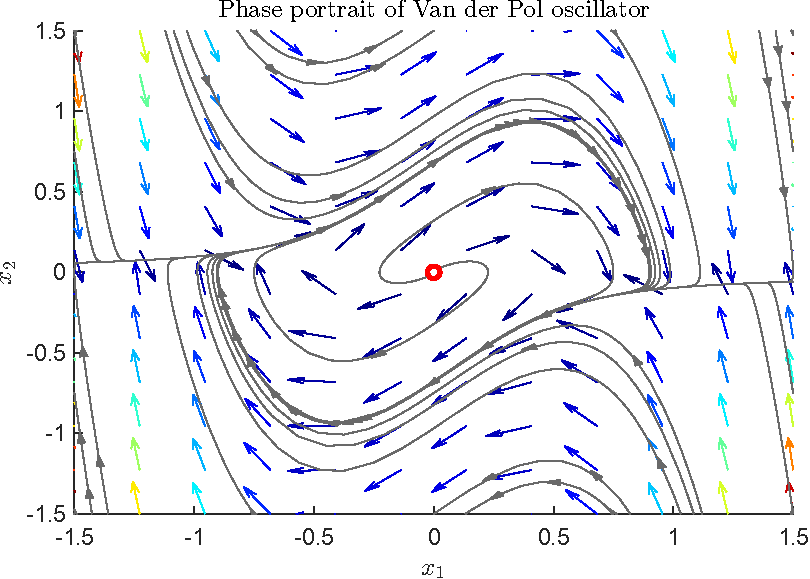
\includegraphics[width=0.6\columnwidth]{figures/vdp/phase_portarit}
    % \caption{Phase portrait of the unforced Van der Pol oscillator}
    \label{fig:pp_vdp}
\end{figure}
\end{frame}

\begin{frame}{Validation of Van der Pol Oscillator Learning}
    \begin{figure}[!tbp]
        \centering
        \subfloat[GP model validation]{\includesvg[width=0.45\columnwidth]{figures/vdp/gp_valdation_w_uncert}\label{fig:f1}}
        \centering
        \subfloat[Moment Matching model validation]{\includesvg[width=0.55\columnwidth]{figures/vdp/long_w_uncert}\label{fig:f1}}
    \end{figure}
\end{frame}


\begin{frame}{Van der Pol oscillator Without Uncertainty}
        \begin{figure}[!tbp]
        \centering
        \subfloat[GP-MPC controller $t_s=13$]{\includesvg[width=0.485\columnwidth]{figures/vdp/GP_mpc_vdp_det}\label{fig:f1}}
        \centering
        \subfloat[f-MPC controller $t_s=10$]{\includesvg[width=0.515\columnwidth]{figures/vdp/f_mpc_vdp_det}\label{fig:f1}}
    \end{figure}
\end{frame}


\begin{frame}{Van der Pol oscillator With Uncertainty}
\[\dot{x}_1 &= (2+2\lambda)x_2 \] 
        \[ \dot{x}_2 &= -(0.8+0.8 \alpha)x_1 + (2+2 \lambda)x_2 - (10+10\gamma)x_1^2x_2 + u\]
    \begin{figure}[!tbp]
        \centering
        \subfloat[GP-MPC controller $t_s=13$]{\includesvg[width=0.35\columnwidth]{figures/vdp/2_Gp_mpc_uncert_vdp}\label{fig:f1}}
        \centering
        \subfloat[f-MPC controller $t_s=9$]{\includesvg[width=0.38\columnwidth]{figures/vdp/2_f_mpc_uncert_vdp}\label{fig:f1}}
    \end{figure}
\end{frame}

\begin{frame}{Reference Tracking $x_f= [-0.25,0]$}
% \includesvg[width=0.1\columnwidth]{figures/vdp/Ref_track_pt_1}
% \includesvg[width=0.485\columnwidth]{figures/vdp/2_setpoint_gp_mpc}
% \includesvg[width=0.515\columnwidth]{figures/vdp/2_fmpc_setpont}
    \begin{figure}[!tbp]
        \subfloat{\includesvg[width=0.16\columnwidth]{figures/vdp/Ref_track_pt_1}}
        
        \subfloat[GP-MPC controller $t_s=13$]{\includesvg[width=0.35\columnwidth]{figures/vdp/2_setpoint_gp_mpc}\label{fig:f1}}
        \centering
        \subfloat[f-MPC controller $t_s=9$]{\includesvg[width=0.38\columnwidth]{figures/vdp/2_fmpc_setpont}\label{fig:f1}}
    \end{figure}
\end{frame}

\begin{frame}{Reference Tracking $x_f= [1,0]$}
        \begin{figure}[!tbp]
        \subfloat{\includesvg[width=0.16\columnwidth]{figures/vdp/phaseportatrit_2}}
        
        \subfloat[GP-MPC controller $t_s=14$]{\includesvg[width=0.38\columnwidth]{figures/vdp/5_gp_mpc_set_1_0}\label{fig:f1}}
        \centering
        \subfloat[f-MPC controller $t_s=12$]{\includesvg[width=0.4\columnwidth]{figures/vdp/5_f_mpc_set_1_0}\label{fig:f1}}
    \end{figure}
\end{frame}

% \begin{frame}{Frame Title}
    
% \end{frame}

% \begin{frame}{Frame Title}
    
% \end{frame}

\section{Conclusion and Outlook}

\subsection{Conclusion}
    \begin{frame} \frametitle{Conclusion}
    \begin{itemize}
        \item Validated GP and Moment Matching Prediction Model - model errors in horizon end 
        % \item Probabilistic MPC using Gaussian processes for Non linear systems. 
        \item DC Motor Model- GP-MPC controller closely resembles f-MPC controller
        \item Precise and faster control in noise-free scenarios of DC motor system
        \item Van der Pol Oscillator- initial struggle to control, satisfactory performance later
        \item Reference tracking of the non linear system to desired point
        \item GP-MPC controller is faster( within $t_s=15$) 
        \item Non-linear model based learning with non linear controller
        \item GP-MPC controller is data efficient (requires 20-50)
        % \item Computationally faster 
        \item Single data-driven controller framework for variety of systems with good performance 
    \end{itemize}
    \end{frame}

\subsection{Outlook}
    \begin{frame}
        \frametitle{Outlook}
\begin{itemize}
    \item Optimize the Moment Matching model for speed and accuracy using advanced modeling techniques and algorithmic improvements
    \item Explore the application of GP-MPC in Multi-Input Multi-Output (MIMO) systems
    \item Implementation GP-MPC framework to real-world systems, including both linear and nonlinear systems
\end{itemize}
    \end{frame}

%%#########################  Final Slide #######################################

\begin{frame}
	\frametitle{The End}
	\centering
	Thank you very much for your attention!
\end{frame}

%%#########################  Appendix    #######################################

\appendix
\section[References]{References long Title}
\begin{frame}
        \footnotesize
	\printbibliography

\end{frame}
% \section[References]{References long Title}
% \begin{frame}
%     \footnotesize
%     \begin{multicols}{2}
%         \footnotesize
%         \printbibliography
%     \end{multicols}
% \end{frame}

\section{Appendix}
\begin{frame}
    \frametitle{GP prior}
    assumes a prior that function values behave according to
    \begin{equation}\label{eq:prior_function}
        p(f | x_1, x_2, \ldots, x_n) = \mathcal{N} (0, K(\mathbf{x_1},  \mathbf{x_2})), 
    \end{equation}
    where $f = [f_1, f_2, \ldots, f_n]^{\top}$ is a vector of latent function values, $f_i = f(\mathbf{x_i})$, and $K(\mathbf{x_1}, \mathbf{x_2})$ is a covariance matrix, whose entries are given by the covariance function, $K(\mathbf{x_1}, \mathbf{x_2})_{ij} = k(\mathbf{x_i}, \mathbf{x_j})$.
    \begin{equation}\label{eq:covariance_function}
        K_{ij} = k(\mathbf{x_i}, \mathbf{x_j}) = \sigma_f^2 \exp\left( -\frac{(\mathbf{x_i} - \mathbf{x_j})^2}{2l^2} \right),
    \end{equation}
    where $\sigma_f^2$ controls the prior variance, and $l$ is an isotropic lengthscale parameter that controls the rate of decay of the covariance

\end{frame}

\begin{frame}{Gaussian Process Regression}
    \begin{itemize}
        \item Ex 1, \(x^* = [0,1]^T \) , \( f(x^*) = [0, 0] \), \(\mathcal{N}\left(\begin{bmatrix}0 \\0\end{bmatrix}, \begin{bmatrix}1 & 0.607 \\0.607 & 1 \end{bmatrix}\right)\)
        \item Ex 2, \(x^* = [0,2]^T \) , \( f(x^*) = [0, 1] \), \(\mathcal{N}\left(\begin{bmatrix}0 \\1\end{bmatrix}, \begin{bmatrix}1 & 0.135 \\0.135 & 1 \end{bmatrix}\right)\)
    \end{itemize}
        \begin{figure}[!tbp]
        \centering
        \includesvg[width=0.6\columnwidth]{figures/GP/bivariateGD}\label{fig:f1}
    \end{figure}
    
\end{frame}

\begin{frame}{Maximizing Marginal likelihood Method}
    Following the GP assumption, the distribution of the training outputs is
given as

\begin{equation}
p(y|X, \theta) = \mathcal{N} (0, \Sigma_{\theta}),
\end{equation}

where $\Sigma_{\theta} = K + \sigma^2_n I$ and $\theta$ is the collection of the unknown hyperparameters. Therefore, the negative log marginal likelihood (nlml) is

\begin{equation}
L(\theta) = - \log p(y|X, \theta) = \frac{1}{2} y^T \Sigma^{-1}_{\theta} y + \frac{1}{2} \log \det \Sigma_{\theta} + \frac{n}{2} \log 2\pi,
\end{equation}

and the partial derivatives of nlml with respect to the hyperparameters are given
by

\begin{equation}
\frac{\partial}{\partial \theta_i} L(\theta) = \frac{1}{2} \mathrm{tr} \left( \Sigma^{-1}_{\theta} \frac{\partial \Sigma_{\theta}}{\partial \theta_i} \right) - \frac{1}{2} y^T \Sigma^{-1}_{\theta} \frac{\partial \Sigma_{\theta}}{\partial \theta_i} \Sigma^{-1}_{\theta} y.
\end{equation}

\end{frame}





\begin{frame}{Moment Matching Approximation}

\begin{itemize}
    \item Alternatively, the posterior distribution \( p(f|x, \mathbf{X}, \mathbf{D}) \) can be approximated as a Gaussian by calculating its mean and variance.
    \item Several methods exist for this Gaussian approximation, such as Moment Matching and linearization of the posterior GP mean function. %\cite{marc2015robotics}.
    \item Moment Matching computes the first two moments of the predictive distribution exactly, whereas linearization provides a computationally efficient approximation by explicitly linearizing the posterior GP.
    \item Moment Matching is better than linearization, we will focus on the Moment Matching Gaussian approximation.
\end{itemize}
\end{frame}

\begin{frame}{Mean Prediction}
    Following the law of iterated expectations, for target dimensions \( a = 1,..., D \) we obtain the predictive mean:

\begin{equation}\label{eq:mu}
\begin{aligned}
\mu_t^a & =\mathbb{E}_{\tilde{\boldsymbol{x}}_{t-1}}\left[\mathbb{E}_{f_a}\left[f_a\left(\tilde{\boldsymbol{x}}_{t-1}\right) \mid \tilde{\boldsymbol{x}}_{t-1}\right]\right]=\mathbb{E}_{\tilde{\boldsymbol{x}}_{t-1}}\left[m_{f_a}\left(\tilde{\boldsymbol{x}}_{t-1}\right)\right] \\
& =\int m_{f_a}\left(\tilde{\boldsymbol{x}}_{t-1}\right) \mathcal{N}\left(\tilde{\boldsymbol{x}}_{t-1} \mid \tilde{\boldsymbol{\mu}}_{t-1}, \tilde{\boldsymbol{\Sigma}}_{t-1}\right) d \tilde{\boldsymbol{x}}_{t-1} \\
& =\boldsymbol{\beta}_a^T \boldsymbol{q}_a 
% \boldsymbol{\beta}_a & =\left(\boldsymbol{K}_a+\sigma_{w_a}^2\right)^{-1} \boldsymbol{y}_a
\end{aligned}
\end{equation}
where, \quad $\boldsymbol{\beta}_a =\left(\boldsymbol{K}_a+\sigma_{w_a}^2\right)^{-1} \boldsymbol{y}_a ,$ \quad \quad $
  \boldsymbol{q}_a=\left[q_{a_1}, \ldots, q_{a_n}\right]^T$. 
\begin{equation}\label{eq:mu_qa}
\begin{aligned}
q_{a_i} & =\int k_a\left(\tilde{\boldsymbol{x}}_i, \tilde{\boldsymbol{x}}_{t-1}\right) \mathcal{N}\left(\tilde{\boldsymbol{x}}_{t-1} \mid \tilde{\boldsymbol{\mu}}_{t-1}, \tilde{\boldsymbol{\Sigma}}_{t-1}\right) d \tilde{\boldsymbol{x}}_{t-1} \\
& =\sigma_{f_a}^2\left|\tilde{\boldsymbol{\Sigma}}_{t-1} \boldsymbol{\Lambda}_a^{-1}+\boldsymbol{I}\right|^{-\frac{1}{2}} \exp \left(-\frac{1}{2} \boldsymbol{\nu}_i^T\left(\tilde{\boldsymbol{\Sigma}}_{t-1}+\boldsymbol{\Lambda}_a\right)^{-1} \boldsymbol{\nu}_i\right),
\end{aligned}
\end{equation}

where we define
\begin{equation}\label{eq:difference_vi}
    \nu_i:=\left(\tilde{\boldsymbol{x}}_i-\tilde{\boldsymbol{\mu}}_{t-1}\right)
\end{equation}
\end{frame}


\begin{frame}{Covariance Matrix Prediction}
    The Predictive covariance matrix $\mathbf{\Sigma}_{\Delta} \in \mathbb{R}^{D \times D}$ is given by 
    \begin{equation}
    \sum (:) = 	\begin{bmatrix}
                        \sigma_{a a}^2 & \sigma_{a b}^2 &......\\
                        \sigma_{a b}^2 & \sigma_{b b}^2 &......\\
                        .&.& ......\\
                        .&.& ......\\
                        \end{bmatrix}_{DxD}
\end{equation}
where, 
\begin{equation}\label{eq:sigma_aa}
\sigma_{a a}^2  =\mathbb{E}_{\overline{\boldsymbol{x}}_t}\left[\operatorname{var}_f\left[\Delta_a \mid \tilde{\boldsymbol{x}}_t\right]\right]+\mathbb{E}_{f, \overline{\boldsymbol{x}}_t}\left[\Delta_a^2\right]-\left(\boldsymbol{\mu}_{\Delta}^a\right)^2,
\end{equation}
\begin{equation}\label{eq:sigma_ab}
    \sigma_{a b}^2 =\mathbb{E}_{f, \overline{\boldsymbol{x}}_t}\left[\Delta_a \Delta_b\right]-\boldsymbol{\mu}_{\Delta}^a \boldsymbol{\mu}_{\Delta}^b, \quad a \neq b,
\end{equation}

\begin{equation}\label{eq:Eab}
\begin{aligned}
\mathbb{E}_{f, \overline{\boldsymbol{x}}_t}\left[\Delta_a \Delta_b\right] & =\mathbb{E}_{\overline{\boldsymbol{x}}_t}\left[\mathbb{E}_f\left[\Delta_a \mid \tilde{\boldsymbol{x}}_t\right] \mathbb{E}_f\left[\Delta_b \mid \tilde{\boldsymbol{x}}_t\right]\right] \\
& {=} \int m_f^a\left(\tilde{\boldsymbol{x}}_t\right) m_f^b\left(\tilde{\boldsymbol{x}}_t\right) p\left(\tilde{\boldsymbol{x}}_t\right) \mathrm{d} \tilde{\boldsymbol{x}}_t \\
& =\boldsymbol{\beta}_a^{\top} \boldsymbol{Q} \boldsymbol{\beta}_b,
\end{aligned}
\end{equation}
\end{frame}

\begin{frame}{Covariance Matrix Prediction}
    
\begin{equation}\label{eq:Q_integral}
    \boldsymbol{Q}:=\int k_a\left(\tilde{\boldsymbol{x}}_t, \tilde{\boldsymbol{X}}\right)^{\top} k_b\left(\tilde{\boldsymbol{x}}_t, \tilde{\boldsymbol{X}}\right) p\left(\tilde{\boldsymbol{x}}_t\right) \mathrm{d} \tilde{\boldsymbol{x}}_t .
\end{equation}

Using standard results from Gaussian multiplications and integration, we obtain the entries $Q_{i j}$ of $Q \in \mathbb{R}^{n \times n}$
\begin{equation}\label{eq:Qij}
    Q_{i j}=|\boldsymbol{R}|^{-\frac{1}{2}} k_a\left(\tilde{\boldsymbol{x}}_i, \tilde{\boldsymbol{\mu}}_t\right) k_b\left(\tilde{\boldsymbol{x}}_j, \tilde{\boldsymbol{\mu}}_t\right) \exp \left(\frac{1}{2} \boldsymbol{z}_{i j}^{\top} \boldsymbol{T}^{-1} \boldsymbol{z}_{i j}\right)
\end{equation}

where we define
$\qquad \boldsymbol{R}  :=\tilde{\boldsymbol{\Sigma}}_t\left(\boldsymbol{\Lambda}_a^{-1}+\boldsymbol{\Lambda}_b^{-1}\right)+\boldsymbol{I}, \qquad \boldsymbol{T}:=\boldsymbol{\Lambda}_a^{-1}+\boldsymbol{\Lambda}_b^{-1}+\tilde{\boldsymbol{\Sigma}}_t^{-1}, \\ \boldsymbol{z}_{i j} :=\boldsymbol{\Lambda}_a^{-1} \boldsymbol{\nu}_i+\boldsymbol{\Lambda}_b^{-1} \boldsymbol{\nu}_j,$

From (\ref{eq:sigma_aa}), we see that the diagonal entries contain the additional term
\begin{equation}\label{eq:E_xa}
\mathbf{E}_{\overline{\boldsymbol{x}}_t}\left[\operatorname{var}_f\left[\Delta_a \mid \tilde{\boldsymbol{x}}_t\right]\right]=\sigma_{f_a}^2-\operatorname{tr}\left(\left(\boldsymbol{K}_a+\sigma_{w_a}^2 \boldsymbol{I}\right)^{-1} \boldsymbol{Q}\right)+\sigma_{w_a}^2
\end{equation}
 $\sigma_{w_a}^2$ being the system noise variance of the $a$th target dimension. 
\end{frame}

%%%%%%%%%%%%%%%%%%%%%%%%%%%%%%%%%%%%%%%%%%%%%%%%%%%%%%%%%%%%%%%%%%%%%%%%%%%%%%%%%%%%%%%%%%%%%%%%%%%






\end{document}